% old version of lit review, before merging with introduction

\chapter{Background and existing work}

In this chapter, we present an overview of the main ideas pertaining to the project. The ultimate aim is to test if jointly aligned embeddings are superior to independently learned embeddings; that is, if the data from one mode will induce better embedding quality in the other mode. 

\section{Concepts}

In this document we will focus on the definition from \cite{stanfordconcepts} of a concept as a mental representation or psychological entity, as it is also a main definition used in cognitive science \cite{Pinker2007}. In \cite{NatureOfHumanConcepts}, concepts are related to human characterisation of categories of objects, noting that categories may overlap and have fuzzy boundaries. In \cite{GOLDSTONE2002295}, concepts are defined not only by features (apple maps to ``red or green or yellow in colour", ``round in shape") - the ``external grounding" description of meaning, but also by their relationships to each other (``apple" is more like ``pear" but less like ``strawberry"). The ``conceptual web" description states that a concept's meaning is defined by its place within the entire structure formed by all concepts. 

In the field of computer science, there exist many frameworks of concepts defined in machine-interpretable ways. Some examples are Cyc \cite{Cyc} (an ontology of ``common-sense" rules and concepts), WordNet (a lexical database of English words, with the inherent assumption that words and concepts are interchangeable) \cite{WordNet}, and the Google Knowledge Graph \cite{KnowledgeGraphs}. These store the connections between concepts like hierarchy and inference, not just names; therefore, a central idea is that these relationships contain valuable information. 

There is precedent for this way of thinking in the psychological and cognitive science literature. \cite{SHEPARD19701} found that the connections between concepts (internal mental representations) should reflect the connections between the external (real world) representations; this was experimentally tested by querying subjects on the identification of US states by shape, and further confirmed by \cite{SecondOrderIsomorphismFaces}, testing the identification of faces. \cite{GOLDSTONE2002295} found an algorithm that was able to use the internal relationships between concepts in disparate systems to find correspondence between those two systems. 

\cite{CoocurrenceVisionLanguage2021} found that object representations in the human brain (which can be thought of as concepts - mental representations) are related to the co-occurrence statistics of objects occurring in images and described in language. They posit that objects occur in context, with certain objects occurring together more often than not, and that the brain possesses mechanisms to support this type of contextual knowledge. They found that brain response as measured by fMRI activity can be predicted by the co-occurrence statistics of objects within a visual scene. \cite{STANSBURY20131025} also found that the brain's response to scenes could be predicted based on clusters of co-occurring objects in that scene. 

Therefore, research evidence suggests that concepts may be considered to embody observed phenomena or events in the world, and that the relationships between concepts are important. 

\section{Embeddings}

In machine learning, embeddings are continuous real-valued vector representations of features. Language embeddings (built from textual input data) are the most commonly known type of embedding, but embeddings may be constructed from any data source. Embeddings are a form of dimensionality reduction. For example a one-hot representation of words in a corpus may have dimensionality in the millions, but converting these to word embeddings might reduce the problem dimensionality to several hundred. One of the earliest word embedding algorithms is \texttt{word2vec} \cite{word2vec}, in which a neural network is used to learn embeddings from a corpus by projecting similar words to similar locations in the target vector space. This algorithm takes advantage of co-occurrence patterns (some words occur in the neighbourhood of other words). The resulting embeddings should reflect the semantic properties of words. The ``Continuous Bag Of Words" (CBOW) variant uses a window of context (disregarding order) to predict the current word, and the Skip-gram variant uses the current word to predict the context window, weighted by distance from the current word. In both cases, we see that the context of the current word is important, pointing again to a relationship between the concepts being used as input into embedding creation. 

The GloVe \cite{pennington2014glove} embedding algorithm is also based on co-occurrence statistics. The co-occurrence of a pair of words is the number of times those words occur within a set context window of each other. The GloVe algorithm attempts to learn embeddings whose dot products give rise to the particular co-occurrence statistics of the corpus. These algorithms can be generalised to learn embeddings from any source of co-occurrence statistics, not just words; in \cite{CoocurrenceVisionLanguage2021}, a set of object embeddings called \texttt{object2vec} was built from co-occurrence statistics from the ADE20K data set \cite{ADE20K} of images labelled by human annotators, using the \texttt{word2vec} algorithm. 

%BERT \cite{BERT}, ELMo \cite{ELMo} and fastText \cite{FastText} take the use of context one step further, in that word embeddings in these models may have different representations for the same word depending on the specific context a word is used. These capture more distant long-range connections between words. This is in contrast to GloVe and \texttt{word2vec}, in which there is only one embedding for any given word and all of its uses in every context in the corpus are taken into account when creating that single embedding. 

\cite{MikolovMachineTranslation} found that word embedding spaces have similar structure over different languages, even when those languages are linguistically quite far apart, like English and Vietnamese- another example of how the relationships between nodes in the concept systems are significant. 

The Laplacian eigenmap algorithm \cite{LaplacianEigenmaps} is a geometrically motivated graph-based algorithm for learning embeddings without using co-occurrence data. A weighted graph is created with a node for each concept/feature, and edges are added between nodes if they meet some definition of closeness (such as Euclidean distance, or being in the $k$-nearest neighbour set). The embeddings are the eigenvectors of the graph Laplacian. This algorithm is also context-based but in a different way; it preserves information about the local neighbourhood geometry. 

Most algorithms for generating embeddings have significant stochasticity, as the learning process often involves minimising loss using stochastic gradient descent. The loss function landscapes are complex with many local minima, and the solution is sensitive to initial conditions. Therefore, runs with different random seeds will produce different embeddings; not just the individual embedding values will differ, but also the relationships between those embeddings. In a later part of this document we show examples of this. 

All of the above algorithms result in point estimates, which are deterministic in the sense that each concept is represented by one vector of numbers. We can generalise the idea to probabilistic embeddings, in which each embedding is represented by multiple vectors that represent parameters of a distribution. For example we may consider embeddings to be multivariate Gaussians with independent dimensions (diagonal covariance matrix), therefore representing each embedding with two $n$-dimensional vectors, for the mean and variance respectively. By learning the variance as well, we derive further information about each concept that can be used to quantify the degree of uncertainty of that concept in the system. When the embeddings are used, a sample is taken from the distribution of each concept whose embedding is desired. \cite{ProbabilisticEmbeddingsCrossModal} represent cross-modal embeddings as probability distributions in embedding space, and use the uncertainty represented by the learned variance in automated decision making. Including the uncertainty in their information retrieval task improved performance, as well as increasing the interpretability of the final embeddings. Looking ahead to the problem of finding correspondences between embeddings in multiple domains, we also see that variance can provide additional information for disambiguation during the mapping process. 

\cite{DensityMatchingWordEmbeddings} and \cite{vilnis2015word} learn word embeddings by modeling each embedding as a probability density function. \cite{DensityMatchingWordEmbeddings} learn bilingual embeddings in an unsupervised way by matching the densities of the two monolingual embedding spaces. This allowed them to achieve state-of-the-art results on linguistically distant language pairs without the special initialisation or complicated optimisation required by many unsupervised methods. \cite{vilnis2015word} learn a mapping from individual words, as well as words in context, to a Gaussian distribution over a latent space. This mapping is such that the linguistic and semantic properties of the words are preserved by the relationships between the distributions. Words that appear in similar context should have similar embeddings. In particular, they wanted entailment relationships (if there is an entailment relationship between A and B, A must imply B) to be represented by inclusion between the variances of the words' respective Gaussian distributions. 

\section{Multi-task learning}

Human learning often follows the multi-task paradigm, where we apply knowledge to one task that was obtained from learning related tasks. Most of us learned arithmetic in primary school, and we apply that to checking the transactions of our bank account, or to adding up the total at the supermarket till. Basic skills are built upon to allow more complex techniques to be learned. 

In the machine learning context, \cite{OverviewMultiTaskLearning} gives several reasons for why multi-task learning allows models to generalise better. By training on multiple tasks, the model can learn a more general representation of the pattern that underlies all those tasks. If this general representation is closer to the true universal generative representation, it will allow the model to generalise to novel tasks better (partially overcoming the bias-variance tradeoff). %Ideally, information from one task's domain should help training for other tasks on other domains.

By learning from multiple tasks simultaneously, we are using more data than we would be by learning a single task. Training a model requires learning a good generalisation for the task that ignores the noise in the data. As different tasks have different patterns of noise, learning multiple simultaneous tasks should allow learning of a more general representation. This reduces the risk of overfitting to only one task. There is also a regularising effect as multi-task learning adds an inductive bias that makes a model favour some hypotheses over others. In the context of our embedding alignment problem, the inductive bias applied should induce the model to learn concept embeddings for the disparate domains that correspond in certain instances, with the hope that this model is more representative of the ``ground truth" of the real world that generates their co-occurrence statistics. Ideally, the knowledge acquired from one domain would inform the embeddings constructed for the other domain. 

\newpage
\section{Alignment and ways to achieve it}
    
\subsection{Some definitions of alignment}

\subsubsection{Alignment as mapping two spaces to a single latent space}
In its simplest form, alignment requires learning to map between two vector spaces. The notation from \cite{ManifoldLearningTheoryAndApplications} is used here to state the problem, as we find it particularly clear.

If there are two datasets $X$ and $Y$ whose instances all lie on the same underlying manifold $Z$, one version of the alignment problem requires finding functions $f$ and $g$ such that $f(x_i)$ is close  to $g(y_j)$, for some problem-specific definition of distance.

\begin{figure}[H]
    \centering
    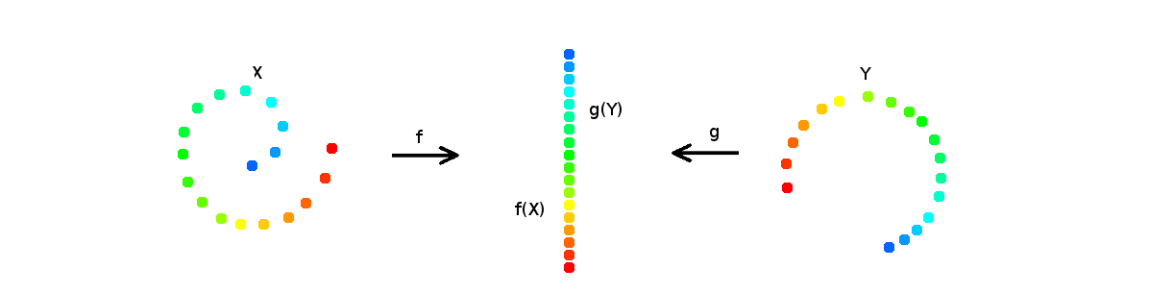
\includegraphics[width=\textwidth]{images/review/alignment.png}
    \caption{
        Figure taken from \cite{ManifoldLearningTheoryAndApplications}. The $\vecX$ and $\vecY$ spirals denote the two datasets, with the center line showing the data points embedded into the shared space, with local similarity relations being preserved. $f$ and $g$ denote the functions mapping $\vecX$ and $\vecY$ respectively into the shared space. 
    }
    % generated by analyse.py 
\end{figure}

If $f(x_i) = g(y_j)$, then $x_i$ and $y_j$ are in correspondence. If we know ahead of time that $x_i$ and $y_j$ are analogous points in their datasets, then we can provide this information to the algorithm that is trying to infer $f$ and $g$. The union of the ranges of $f$ and $g$ is then the joint latent space. This can be generalised to more than two datasets. 

This however is a definition that maps both domains into the same space. 

\newpage
\subsubsection{Alignment as learning mappings from one domain to another}

In the previous definition, alignment requires that both domains be mapped to a single latent domain. This can be useful for certain problems, for example to find a single language-independent representation of the data in multilingual related corpora. There is another definition for alignment, which requires only that domains can be mapped to each other directly. 

\begin{figure}[H]
\label{fig:alignment2}
    \centering
    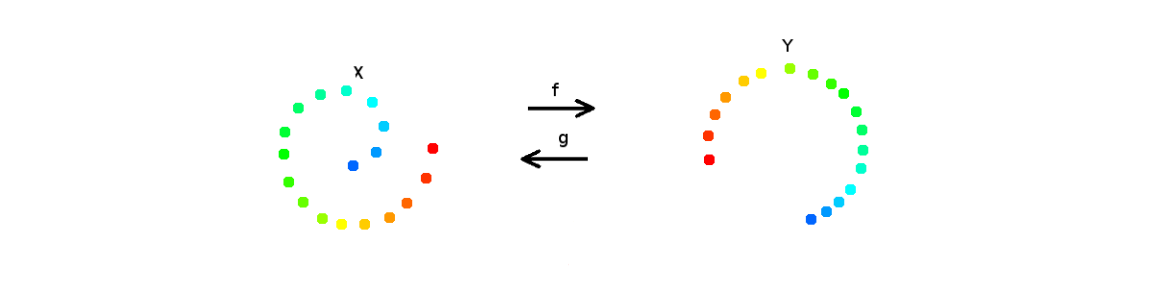
\includegraphics[width=\textwidth]{images/review/alignment2.png}
    \caption{
        The $\vecX$ and $\vecY$ spirals still denote the two datasets, but this time $f$ and $g$ denote the functions mapping $\vecX$ and $\vecY$ respectively to each other, instead of into some shared space.
    }
    % generated by analyse.py 
\end{figure}

We wish to find mappings $f(\vecX) \rightarrow \vecY$ and $g(\vecY) \rightarrow \vecX$ where the spaces $\vecX$ and $\vecY$  have similar structures. This is slightly different from the definition of alignment in the previous section. This definition may be used when it is not clear what the dimensionality of the latent space should be. 

\subsubsection{Second order isomorphism}

Returning to an idea first raised in \cite{SHEPARD19701}, we want second order isomorphism- functional relationships between clusters of concepts over the two modalities. Even if there is no structural resemblance between a concept and that concept's representation, the same structure should be observed between the relationships between the concepts  and the representations. As stated by \cite{GOLDSTONE2002295}, the meaning of a concept is tied to its relationships to other concepts within that modality. Similarity relationships between concepts within the same system can therefore be used to map between systems; using only these relationships, \cite{GOLDSTONE2002295} found an algorithm, ABSURDIST, that was able to translate between concept systems. Without constraints on the two systems, or even on the number of concepts in each system, ABSURDIST was able to find translations using only similarity matrices created by some external agent (for example a German-English bilingual human). ABSURDIST found that while within-system relationships are enough to find a translation, this translation can be made more robust to noise by adding external, extrinsic information about correspondences (for example higher weights for certain correspondences). 

\cite{GOLDSTONE2002295} found that ABSURDIST's mappings were better for systems that had a greater number of elements. This is because such a system has more similarity relations, and each similarity relation provides a constraint to uniquely identify each member. Therefore, systems with more elements are more constrained. 

\subsubsection{Applications of alignment problems}

Some examples of alignment problems are given below. They span a wide range of applications. 

\begin{itemize}
    \item Biological manifold alignment: \cite{magan} applies Generative Adversarial Networks \cite{GAN} to the problem of alignment of cell correspondence between cytometry batches.
    \item Neural style transfer: \cite{CycleGAN} takes as input differently styled source and target image sets and applies adversarial network techniques to translate images from the source set style into the target set style. 
    \item Bilingual lexical induction: \cite{wordtranslationwithoutparalleldata} applies unsupervised alignment between monolingual word representations to derive a dictionary between those languages.
    \item Deep multimodal embedding: \cite{DeepMultimodalEmbedding} relates information from three modalities- point-cloud, natural language and manipulation trajectory data, to teach a robot arm  how to manipulate new objects. 
\end{itemize}

\subsection{Methods for concept alignment}

In this section, the following notation applies:

\begin{equation}
\begin{split}
    \vecX \medspace \text{denotes embeddings in the source domain},\\
    \vecY \medspace \text{denotes embeddings in the target domain},\\
    \vecW \medspace \text{denotes a transformation matrix}.\\
\end{split}
\end{equation}

\subsubsection{Regression and related models}

Regression models are the simplest form of alignment model. They only require learning a transformation matrix $\vecW$ from one domain to another, minimising mean squared loss $|| (\vecW \vecX + \vecb) - \vecY||_2^2$ which can then be applied to a new source vector to map into the target space. \cite{MikolovMachineTranslation} uses this to find a ``translation matrix" that can map from word embeddings in one language space to another. Orthogonal models constrain the learned $\vecW$ matrix to be orthogonal, which is appropriate if the angles between embeddings are more important as a measure of similarity than the distances between them. Various standard preprocessing steps may be applied like normalisation to unit norm / mean centering, decorrelation to have unit variance, or SVD for dimension reduction.

Maximum margin models are similar to the support vector machine \cite{SVM} in that they balance increasing the weights from matching pairs with reducing the weights learned from known generated noise pairs. An example loss function (reproduced from \cite{kalinowski2020survey}) is:

\begin{equation}
\begin{split}
\sumin \sum_{j \neq i}^{k} &\max \{0, \gamma - \cos(\vecW \vece_i^s, \vece_i^t) + \cos(\vecW \vece_i^s, \vece_j^t)\}\\
\spaced{with}& \vece_i, \vece_j \lspaced{being the $i$th and $j$th of $n$ embeddings},\\
& \vecW \lspaced{being the transformation matrix},\\
& k \lspaced{being the number of noise pairs}, \\
& \lspaced{and}\medspace \gamma \lspaced{being the margin parameter}.
\end{split}
\end{equation}

This is different from regression models which rely largely on minimising the mean-squared error. \cite{Hubness} found that this form of loss reduced the effect of hubs that can plague regression and orthogonal techniques. Hubs are embeddings with high similarity to all vectors in the space, due to entities that are too common (such as words that are very frequent in a corpus) or simply as an artifact of the transformation where many features get mapped to a small region of embedding space spuriously. \cite{ImprovingSupervisedBilingualMapping} introduce another metric to reduce hubness, cross-domain similarity local scaling, that incorporates the mean of $k$-nearest neighbour distances of points in the target space to capture the neighbourhood geometry. 

Point set registration, most commonly found in computer vision, is the alignment problem applied to sets of points in 2 or 3 dimensions. \cite{PointSetRegistrationReview} reviews many current techniques; one key difference between this problem and the general alignment problem is that the points are known to lie on a 2- or 3-dimensional manifold, and this is quite a significant constraint. We cannot make any such assumptions about the dimensionality of our embeddings. 

\subsubsection{Manifold alignment models}

As stated in \cite{ManifoldLearningTheoryAndApplications}, manifold alignment is a type of constrained simultaneous dimensionality reduction with the aim of finding a low-dimensional embedding of all input datasets that preserves the topology of correspondences between them. The datasets may have disjoint features. The data may be of very high dimension, but if all the data points lie on a low-dimensional manifold, this manifold may be learnable.  

This requires the multiple datasets to be representable by a shared underlying structure. It may be convenient to learn the mappings between datasets without ever formalising this shared structure, or it may be useful to find common features. For example, in language translation it may be enough to know the mappings from words or phrases in one language to the equivalent entities in another language. However if the problem is multilingual information retrieval, it may be more useful to express the translations of different documents as a single underlying joint representation. Our specific problem is learning aligned embeddings from co-occurrence data that represent the statistics of how concepts occur in different human-created media. If we consider the ultimate underlying generative process of all these media to be ``the real world", it is plausible that the embeddings could have some underlying shared joint representation, but we do not know anything about this representation. In particular, we do not know the dimensionality of the underlying process. 

Some existing dimensionality reduction techniques that can be used in alignment are the Isomap \cite{Isomap}, which reduces dimension while preserving distances between points; locally linear embedding \cite {LocallyLinearEmbedding}, which reduces dimension while keeping distances the same between local neighbourhoods; and the Laplacian eigenmap \cite{LaplacianEigenmaps}, which approximates the manifold by the adjacency graph derived from the embeddings. These algorithms all try to find the low dimensional representation of a single dataset, and manifold alignment simply uses these or similar algorithms to find embeddings for multiple datasets simultaneously. Without correspondence information, manifold alignment will result in independent embeddings for each input dataset, but if direct correspondence information is provided, or a means for inferring it, manifold alignment will use this to constrain the embeddings to be aligned. %Manifold alignment considers each individual dataset to be part of one larger dataset whose range includes the mapped values of all other datasets. 

In \cite{UnsupervisedAlignmentWP}, an approach to aligning two sets of existing embeddings (learned separately from the alignment procedure) using a combination of Procrustes analysis and the Wasserstein distance is described. Procrustes analysis is normally used to learn an affine transformation between two sets of points with a known correspondence. If we consider $\vecX \in \R^{n \times d}$ ($n$ vectors of dimension $d$) and $\vecY \in \R^{n \times d}$ (another set of vectors of the same size), the Procrustes linear transformation is the solution to the following:

\begin{equation}
    \argmin{\vecW \in \R^{d \times d}} \quad  ||\vecX \vecW - \vecY||_2^2
\end{equation}

\cite{Goodall1991ProcrustesMI} used this to analyse two-dimensional shapes, where the shapes are considered to be the same if by application of rotation, translation and isotropic scaling, one can be transformed to the other. \cite{MikolovMachineTranslation} applied this technique to learn linear mappings between word embeddings in different languages using a bilingual dictionary. 

The Wasserstein distance, also known as the Earth Mover Distance, is the solution of the following optimisation problem

\begin{equation}
\begin{split}
    &\argmin{\vecP \in \mathscr{P}_n} \quad || \vecX - \vecP \vecY ||_2^2 \\
    \spaced{where}&\mathscr{P}_n = \{\vecP \in \{0, 1\}^{n \times n}, \vecP \one_n = \one_n, \vecP^T \one_n = \one_n \}
\end{split}
\end{equation}

where $\mathscr{P}_n$ denotes a permutation matrix. It enforces a one-to-one mapping from the rows of $\vecX$ to $\vecY$.

%If the source and target embeddings $\vecX$ and $\vecY$ are thought of as probability distributions, $\mathscr{P}_n$ denotes a permutation matrix that moves mass from $\vecX$ to create $\vecY$. 

\cite{Zhang2017EarthMD} used this distance measure as a minimisation objective to perform automated translation without supervision. By using the Wasserstein distance as a measure of closeness between the source and target embedding spaces, they formulate a system in which minimisation of this distance draws the two distributions closer. %The translation problem faced by \cite{Zhang2017EarthMD} did not have a one-to-one mapping between symbols, because some symbols in one space map to one symbol in the other space, therefore the minimisation of the objective had to be considered over the whole distribution. 

%\cite{UnsupervisedAlignmentWP} combined both Procrustes analysis and the Wasserstein distance, to solve the following optimisation problem:

%\begin{equation}
%\begin{split}
%\argmin{\vecQ \in \mathscr{O}_d} \quad \argmin{\vecP \in \mathscr{P}_n }\quad || \vecX \vecQ - \vecP \vecY||_2^2
%\end{split}
%\end{equation}

%where $\vecQ$ is an orthogonal matrix. In order to practically solve this optimisation, they developed a novel stochastic algorithm to minimise a convex relaxation of this problem, details of which are omitted here. 

\subsubsection{Graph matching and graph similarity methods}

A system of interconnected concepts can be represented as a graph whose nodes represent concepts and whose edges (which may be weighted) represent relationships between concepts. For example, in \cite{Absurdist2}, such a system is represented as a directed graph with $N$ nodes whose edges are connected with labels from the set $S$ representing all combinations of possible relationships between any two nodes. Examples of such relations are ``Similar to", ``Is-A" or other hyponymic / synonymic relationships, or weights corresponding to the degree of co-occurrence of the two concepts. \cite{Absurdist2}, a sequel to \cite{GOLDSTONE2002295}, further describes how alignment of two conceptual systems may be formalised as matching two graphs.

The general graph isomorphism problem, that of telling if two graphs represent the same structure, is NP-hard \cite{GraphIsomorphismNPHard}. As cited in \cite{Absurdist2}, much work has been done in the field of finding approximate isomorphisms; finding a function $s(.)$ such that for two graphs $G_1$ and $G_2$, the distance between $s(G_1)$ and $s(G_2)$ is minimised, where $s$ is a problem-specific distance measure. There are polynomial-time algorithms for certain subtypes of graphs or trees, but in general heuristic algorithms are the only practical possibilities. 

The ABSURDIST II algorithm described in \cite{Absurdist2} creates a matrix of feasible translations between the two concept graphs which is iteratively updated based on the similarity between distances between elements of the system. At the end of the iterations, the output is a correspondence matrix that describes the strength of correspondence between elements of the source and target sets; this is used to create the mapping from source to target items. 

The \texttt{torch-two-sample} Python library and its corresponding paper \cite{torchtwosample} introduce smoothed versions of some graph-based similarity measures, such as the Friedman-Rafsky test and k-nearest neighbours test, that can be used as loss functions for learning similar graph structures. These are not actual graph isomorphism methods, but rather aim to provide distributional similarity metrics based on graph-based properties. These are converted to smooth functions by taking the statistics to be expectations of a probability distribution, thus allowing implementations to be used as loss functions trainable by backpropagation. %Further details may be found in the appendix (\ref{appendix:graphbased}). 

\subsubsection{Generative adversarial networks}

The ``generative" part of a generative adversarial model is a function (usually learned by a deep learning network) that outputs samples from a distribution indistinguishable from a particular input dataset. A discriminator model is then trained against the generated outputs so that it learns to tell the difference between real and synthetic outputs; this is the ``adversarial" part. By alternating the training of these two models, the generator learns to produce better and better samples. In effect, the generator is learning to produce samples from the manifold on which the input data lies. This model was first introduced in \cite{GAN} and while the main objective is usually to generate new samples from a given distribution, there are examples where it has been used for alignment.

The Manifold Alignment GAN \cite{magan} attempts to counteract some of the problems with traditional GANs, one of them being that generated items can fool the discriminator at a batch level because the two manifolds are superimposed, rather than being aligned. When the manifolds are superimposed rather than aligned, it is as if the ``edges" of the manifolds match, but the points within may be in any position. If we were to overlay the manifolds, the corresponding points would not overlap. There are an exponential number of possible mappings that result in overlapping but unaligned manifolds. The MAGAN introduces a correspondence loss that measures the distance between a data point and its mapped image in the other domain, as well as the reconstruction loss (difference between an original point and its reconstructed image after going through both generators). %It also uses the mini-batch discrimination technique described in \cite{ImprovedTechniquesTrainingGANS} to prevent mode collapse, where all inputs get mapped to the same embedding by the generator.

%\cite{wordtranslationwithoutparalleldata} presents an adversarial method for learning cross-lingual word embeddings without supervision (without knowing beforehand any correspondences between the languages). If we consider the usual notation of $\vecX$ being the source embedding space and $\vecY$ being the target embedding space, the objective is to learn $\vecW$ such that $\vecW \vecX$ and $\vecY$ are as similar as possible. The discriminator is trained to distinguish between random samples from $\vecW \vecX$ and $\vecY$, while the generator is trained to learn $\vecW$ to prevent the discriminator from predicting accurately. They found however that the adversarial method alone did not yield better results than the supervised baseline. Therefore they also adopted a refinement procedure using Procrustes analysis to further improve the learned $\vecW$. They found that the adversarial approach would try to align all words even if they are not frequent, but the embeddings for rare words are then less frequently updated. Since the learned mapping is linear ($\vecW \vecX$) it would make sense to learn the mapping using only the most frequent words and refine afterwards. They also used the cross-domain similarity local scaling metric, which uses nearest neighbour information of each embedding to provide additional information to the optimisation.

CycleGAN \cite{CycleGAN} is not specifically an alignment model, but contains useful features. CycleGAN is intended to provide image-to-image translation, where given two unordered image collections, one can be ``translated" into the style of the other. For example, transforming pictures in the style of Monet into photographic style images. CycleGAN contains two GANs; one learns a mapping $f$ from the input set $\vecX$ to the target set $\vecY$, and one learns the mapping $g$ which maps $\vecY$ to $\vecX$. A key part of the CycleGAN model is the cycle consistency loss, which for the domain $\vecX$ is $f(g(\vecY)) - \vecX$ (there is an equivalent cycle consistency loss going the other way). This loss is intended to induce $f$ and $g$ to be consistent with each other; the MAGAN model also uses this loss, calling it ``reconstruction loss". The cycle consistency / reconstruction loss is intended to reduce the possibility of the learned mapping distribution matching the output distribution, but individual inputs not being mapped to individual outputs, a different way of expressing the alignment problem. 

While GANs provide a useful basis for some alignment problems, certain types of datasets are better suited as inputs. Datasets with large numbers of object classes are not suited to GANs as they tend to underestimate the entropy in the distribution \cite{ImprovedTechniquesTrainingGANS}. Many GAN implementations take images as input, and generally the input datasets are very large, providing many samples from which to learn the appropriate distribution. Our particular dataset could be considered to have only one stimulus per concept, if we take all concepts as end nodes in the taxonomy tree.  Additionally, the salient features of images are more likely to lie on 2- or 3-dimensional manifolds, and convolutional architectures are well placed to handle detecting these. We do not know the appropriate dimensionality for the distribution that would represent any underlying manifold the concept embeddings may lie on; if the dimension of the GAN's latent space is not adequate, it will not be able to explore the sample space well, and learning will not occur. 

\todo[inline]{Add summary paragraph as per BR comment: "might want to add a concluding paragraph that summarizes the general weaknesses of existing approaches and briefly re-state why our method is interesting given these existing weaknesses"}
